% !Tex Program = pdflatex

\documentclass[openany,twoside,12pt]{book}
%\documentclass[twoside,12pt]{book}

%----- Packages for template -----
\usepackage{amsmath,amsthm,amssymb}
\usepackage{mathrsfs,bm}
%\usepackage[notcite,notref]{showkeys}
\usepackage{geometry}
\geometry{left=2.5cm,right=2.5cm,top=3.0cm,bottom=3.0cm}
%\geometry{left=1in,right=1in,top=1in,bottom=1in}
%\geometry{left=2.5cm,right=2.1cm,top=1.7cm,bottom=2cm,includehead,includefoot}
%\geometry{b5paper,text={125mm,195mm},centering,left=1in,right=1in,top=1in,bottom=1in}

\usepackage[english]{babel}
\usepackage{imakeidx}
\usepackage{color,xcolor}
\usepackage{graphicx}
\usepackage{epsfig}
\usepackage{tabularx,array}
\usepackage{longtable}
\usepackage{booktabs}
\usepackage{enumitem}
\usepackage{multirow}
\usepackage{multicol}
\usepackage{fancybox}
\usepackage{makecell}
\usepackage{algorithm}
\usepackage{algorithmicx}
\usepackage{algpseudocode}
\usepackage{xstring}
%\usepackage[english]{babel}
\usepackage{listings}
\usepackage{titletoc}
\usepackage{titlesec}
\usepackage{mathtools}
\usepackage{float}
\usepackage{bookmark}

% package for bibliography support
\usepackage[numbers,sort&compress]{natbib}

%\usepackage{indentfirst}
\usepackage[perpage,symbol]{footmisc}   % footnote setting

\usepackage{url,hyperref}
\hypersetup{
  colorlinks = true,
  linkcolor = black,
  citecolor = black,
  filecolor = blue,
  urlcolor =blue,
}

% caption setting
\usepackage{caption}
%\captionsetup{font={small,singlespacing},labelformat={default},labelsep=period}
\captionsetup[figure]{position=bottom,skip={5pt},name={Figure}}
\captionsetup[table]{position=top,skip={2pt},name={Table}}
%\setlength{\textfloatsep}{12pt plus 2pt minus 2pt}
%\setlength{\floatsep}{10pt plus 2pt minus 2pt}
%\setlength{\intextsep}{10pt plus 2pt minus 2pt}
%\setlength{\abovecaptionskip}{2pt plus 1pt minus 1pt}
%\setlength{\belowcaptionskip}{3pt plus 1pt minus 2pt}

\makeindex
%\bibliographystyle{plain}

%---- header and footer position -----
%\setlength{\headheight}{18pt}
%\setlength{\headsep}{18pt}
%\setlength{\footskip}{28pt}

%---- Contents Setting -----
\setcounter{tocdepth}{3}
\setcounter{secnumdepth}{3}


\usepackage[cleardoublepage=plain]{scrextend}

\usepackage{fancyhdr,fancyref}
\pagestyle{fancy}
%\renewcommand{\chaptermark}[1]{\markboth{\thechapter ~ #1}{}}
%\renewcommand{\sectionmark}[1]{\markright{\thesection ~ #1}{}}
\fancyhf{}  % remove the original style
\fancyhead[RO,LE]{~\thepage~}
\fancyhead[LO]{\rmfamily \rightmark}
\fancyhead[RE]{\rmfamily \leftmark}

\setlength{\headheight}{15pt}
%\setlength{\parskip}{3pt plus1pt minus1pt}

\renewcommand{\baselinestretch}{1.2}

%----- theorem setting -----
\theoremstyle{plain}
\newtheorem{definition}{Definition}[chapter]
\newtheorem{proposition}{Proposition}[chapter]
\newtheorem{lemma}{Lemma}[chapter]
\newtheorem{theorem}{Theorem}[chapter]
\newtheorem{example}{Example}[chapter]
\newtheorem{corollary}{Corollary}[chapter]
\newtheorem{remark}{Remarks}[chapter]
\newtheorem{exercise}{Exercise}[chapter]
\newtheorem{assumption}{Assumption}[chapter]
\newtheorem{axiom}{Axiom}[chapter]
\newtheorem{property}{Property}[chapter]
\newtheorem{conjecture}{Conjecture}[chapter]
%\renewcommand{\proofname}{Proof}

% new command for tabularx
\newcolumntype{L}{X}
\newcolumntype{C}{>{\centering \arraybackslash}X}
\newcolumntype{R}{>{\raggedleft \arraybackslash}X}
\newcolumntype{P}[1]{>{\centering \arraybackslash}p{#1}}

% number of equation, figure and table
\numberwithin{equation}{chapter}
\numberwithin{figure}{chapter}
\numberwithin{table}{chapter}

% define new command
\newcommand{\CC}{\ensuremath{\mathbb{C}}}
\newcommand{\RR}{\ensuremath{\mathbb{R}}}
\newcommand{\A}{\mathcal{A}}
\newcommand{\ii}{\bm{\mathrm{i}}\,}  % imaginary part
\newcommand{\md}{\mathrm{d}\,}
\newcommand{\bA}{\boldsymbol{A}}
\newcommand{\red}[1]{\textcolor{red}{#1}}

\newcommand{\plogo}{\fbox{$\mathcal{PL}$}} % Generic dummy publisher logo

\graphicspath{{./figure/}{./figures/}{./image/}{./images/}}


%----- Book information -----

\title{\bfseries LaTeX Book Sample}
\author{Edited by Andy}
\date{February 2023}


\begin{document}

\maketitle

\thispagestyle{empty}

\frontmatter


\chapter{Preface}

The quick brown fox jumps over the lazy dog. The quick brown fox jumps over the lazy dog. The quick brown fox jumps over the lazy dog. The quick brown fox jumps over the lazy dog. The quick brown fox jumps over the lazy dog. The quick brown fox jumps over the lazy dog. The quick brown fox jumps over the lazy dog. The quick brown fox jumps over the lazy dog. The quick brown fox jumps over the lazy dog.


The quick brown fox jumps over the lazy dog. The quick brown fox jumps over the lazy dog. The quick brown fox jumps over the lazy dog. The quick brown fox jumps over the lazy dog. The quick brown fox jumps over the lazy dog. The quick brown fox jumps over the lazy dog. The quick brown fox jumps over the lazy dog. The quick brown fox jumps over the lazy dog. The quick brown fox jumps over the lazy dog.



%\clearpage
\cleardoublepage
\phantomsection
\pdfbookmark[chapter]{\contentsname}{toc}
\tableofcontents


\mainmatter



\chapter{The first chapter}

\section{The first section}\label{my label}
LaTeX is a high-quality typesetting system; it includes features designed for the production of technical and scientific documentation. LaTeX is the de facto standard for the communication and publication of scientific documents.

The unnumbered list
\begin{itemize}
  \item item one
  \item item two
  \item item three
\end{itemize}

The numbered list
\begin{enumerate}
  \item item one
  \item item two
  \item item three
\end{enumerate}

\subsection{A sub section}
LaTeX is not a word processor! Instead, LaTeX encourages authors not to worry too much about the appearance of their documents but to concentrate on getting the right content. For example consider this document:
\begin{equation}\label{eqn:trifun}
\sin^2{\theta}+\cos^2{\theta}=1.
\end{equation}

LaTeX is based on the idea that it is better to leave document design to document designers, and to let authors get on with writing documents.

The \texttt{align} environment
\begin{align}
a & = b + c \\
& = d + e.
\end{align}

Use command \verb|\notag| or \verb|\nonumber| to remove number of equation.
\begin{align}
a ={} & b + c \\
={} & d + e + f + g + h + i + j \notag \\
& + m + n + o \\
={} & p + q + r + s.
\end{align}

The \texttt{gather} environment
\begin{gather}
a = b + c \\
d = e + f + g \notag \\
h + i = j \\
l + m = n
\end{gather}

An example of the \verb|\cite| command to cite within the book:

This statement requires citation \cite{Adams2003} and \cite{Shen1994,Tadmor2012,TreWei2014}


we present a new method for solving the model equation
\begin{equation}\label{eq:mulequ}
\left\{\begin{aligned}
  & \partial_{t} u-\varepsilon^{2} \Delta u+u^{3}-u=0, \quad \text{ in } ~\Omega\times\mathcal{T}, \\
  &\, u(x,y,t) = g(t), \quad \text{ on } ~ \partial \Omega, \\
  &\, u(x,y,0)=\varphi(x, y), \quad \text{ on } ~\Omega.
\end{aligned}\right.
\end{equation}
where $\varepsilon$ is a small parameter.

The quick brown fox jumps over the lazy dog. The quick brown fox jumps over the lazy dog. The quick brown fox jumps over the lazy dog. The quick brown fox jumps over the lazy dog. The quick brown fox jumps over the lazy dog. The quick brown fox jumps over the lazy dog. The quick brown fox jumps over the lazy dog.

The quick brown fox jumps over the lazy dog. The quick brown fox jumps over the lazy dog. The quick brown fox jumps over the lazy dog. The quick brown fox jumps over the lazy dog. The quick brown fox jumps over the lazy dog. The quick brown fox jumps over the lazy dog. The quick brown fox jumps over the lazy dog.


\section{The second section}
LaTeX is a high-quality typesetting system; it includes features designed for the production of technical and scientific documentation. LaTeX is the de facto standard for the communication and publication of scientific documents.

\subsection{A sub section}
LaTeX is not a word processor! Instead, LaTeX encourages authors not to worry too much about the appearance of their documents but to concentrate on getting the right content. LaTeX is a high-quality typesetting system; it includes features designed for the production of technical and scientific documentation. LaTeX is the de facto standard for the communication and publication of scientific documents.

The quick brown fox jumps over the lazy dog. The quick brown fox jumps over the lazy dog. The quick brown fox jumps over the lazy dog. The quick brown fox jumps over the lazy dog. The quick brown fox jumps over the lazy dog. The quick brown fox jumps over the lazy dog. The quick brown fox jumps over the lazy dog. The quick brown fox jumps over the lazy dog. The quick brown fox jumps over the lazy dog.

\begin{definition}
This is a definition environment.
\end{definition}

\begin{lemma}
This is a lemma environment.
\end{lemma}

\begin{theorem}
This is a theorem environment.
\end{theorem}

\begin{proposition}
This is a proposition environment.
\end{proposition}

\begin{lemma}
This is a lemma environment
\begin{enumerate}[label=\rm (\roman*)]
  \item item A
  \item item B
  \begin{equation}\label{eq:limite}
    \lim_{n\to\infty}\left(1+\frac{1}{n}\right)^n=e.
  \end{equation}
\end{enumerate}
\end{lemma}

\begin{theorem}[Mass--energy]
This is a theorem environment.
\end{theorem}
\begin{proof}
  This is a proof environment.
\end{proof}

\begin{remark}
  This is a remark environment.
\end{remark}

\begin{example}
  This is example environment.
\end{example}

The quick brown fox jumps over the lazy dog. The quick brown fox jumps over the lazy dog. The quick brown fox jumps over the lazy dog. The quick brown fox jumps over the lazy dog. The quick brown fox jumps over the lazy dog. The quick brown fox jumps over the lazy dog. The quick brown fox jumps over the lazy dog.

The quick brown fox jumps over the lazy dog. The quick brown fox jumps over the lazy dog. The quick brown fox jumps over the lazy dog. The quick brown fox jumps over the lazy dog. The quick brown fox jumps over the lazy dog. The quick brown fox jumps over the lazy dog. The quick brown fox jumps over the lazy dog.


\section{The third section}
LaTeX is a high-quality typesetting system; it includes features designed for the production of technical and scientific documentation. LaTeX is the de facto standard for the communication and publication of scientific documents.

Here we state our main result as \ref{thm:bigthm}.

\begin{theorem}[$LDL^T$ Factorization \cite{GoVa2013}]\label{thm:bigthm}
  If $A \in \mathbb{R}^{n \times n}$ is symmetric and the principal
  submatrix $A(1:k,1:k)$ is nonsingular for $k=1:n-1$, then there
  exists a unit lower triangular matrix $L$ and a diagonal matrix
  \begin{equation*}
    D = \operatorname{diag}(d_1,\dots,d_n),  %\diag(d_1,\dots,d_n)
  \end{equation*}
  such that $A=LDL^T$. The factorization is unique.
\end{theorem}

LaTeX is a high-quality typesetting system; it includes features designed
for the production of technical and scientific documentation.
LaTeX is the de facto standard for the communication and publication of scientific documents.
LaTeX is based on the idea that it is better to leave document design to
document designers, and to let authors get on with writing documents.

\begin{theorem}[Mean Value Theorem]\label{thm:mvt}
  Suppose $f$ is a function that is continuous on the closed interval
  $[a,b]$.  and differentiable on the open interval $(a,b)$.
  Then there exists a number $c$ such that $a < c < b$ and
  \begin{equation*}
    f'(c) = \frac{f(b)-f(a)}{b-a}.
  \end{equation*}
  In other words,
  \begin{equation*}
    f(b)-f(a) = f'(c)(b-a).
  \end{equation*}
\end{theorem}

\begin{remark}
Observe that \ref{thm:bigthm}, \ref{thm:mvt} correctly mix references
to multiple labels.
\end{remark}

% command cref package cleveref
%Observe that \cref{thm:bigthm,thm:mvt,cor:a} correctly mix references
%to multiple labels.

\begin{corollary}\label{cor:a}
  Let $f(x)$ be continuous and differentiable everywhere. If $f(x)$
  has at least two roots, then $f'(x)$ must have at least one root.
\end{corollary}
\begin{proof}
  Let $a$ and $b$ be two distinct roots of $f$.
  By \ref{thm:mvt}, there exists a number $c$ such that
  \begin{equation*}
    f'(c) = \frac{f(b)-f(a)}{b-a} = \frac{0-0}{b-a} = 0.
  \end{equation*}
\end{proof}

Note that it may require two \LaTeX\ compilations for the proof marks
to show.

Display matrices can be rendered using environments from \texttt{amsmath}:
\begin{equation}\label{eq:matrices}
S=\begin{bmatrix}1&0\\0&0\end{bmatrix}
\quad\text{and}\quad
C=\begin{pmatrix}1&1&0\\1&1&0\\0&0&0\end{pmatrix}.
\end{equation}
Equation \ref{eq:matrices} shows some example matrices.

We calculate the Fr\'{e}chet derivative of $F$ as follows:
\begin{subequations}
\begin{align}
  F'(U,V)(H,K)
  &= \langle R(U,V),H\Sigma V^{T} + U\Sigma K^{T} -
  P(H\Sigma V^{T} + U\Sigma K^{T})\rangle \label{eq:aa} \\
  &= \langle R(U,V),H\Sigma V^{T} + U\Sigma K^{T}\rangle
  \nonumber \\
  &= \langle R(U,V)V\Sigma^{T},H\rangle +
  \langle \Sigma^{T}U^{T}R(U,V),K^{T}\rangle. \label{eq:bb}
\end{align}
\end{subequations}
\ref{eq:aa} is the first line, and \ref{eq:bb} is the last line.

\section{Algorithm}
\label{sec:alg}

Our analysis leads to the algorithm in \ref{alg:buildtree}.

\begin{algorithm}
\caption{Build tree}
\label{alg:buildtree}
\begin{algorithmic}
  \State {Define $P:=T:=\{ \{1\},\ldots,\{d\}$\}}
  \While{$\#P > 1$}
    \State {Choose $C^\prime\in\mathcal{C}_p(P)$ with $C^\prime := \operatorname{argmin}_{C\in\mathcal{C}_p(P)} \varrho(C)$}
    \State {Find an optimal partition tree $T_{C^\prime}$ }
    \State {Update $P := (P{\setminus} C^\prime) \cup \{ \bigcup_{t\in C^\prime} t \}$}
    \State {Update $T := T \cup \{ \bigcup_{t\in\tau} t : \tau\in T_{C^\prime}{\setminus} \mathcal{L}(T_{C^\prime})\}$}
  \EndWhile
  \State \Return $T$
\end{algorithmic}
\end{algorithm}

\clearpage
Adjust the width of the algorithm environment
\begin{center}
\vspace{-2ex}
\begin{minipage}{0.9\linewidth}
\begin{algorithm}[H]
\caption{Euclid’s algorithm}
\label{alg:euclid}
\begin{algorithmic}[1] % line numbering
\Procedure{Euclid}{$a,b$}\Comment{The g.c.d. of a and b}
  \State $r \gets a \bmod b$
  \While{$r\not=0$}\Comment{We have the answer if r is 0}
    \State $a \gets b$
    \State $b \gets r$
    \State $r \gets a \bmod b$
  \EndWhile\label{euclidendwhile}
  \State \textbf{return} $b$\Comment{The gcd is b}
\EndProcedure
\end{algorithmic}
\end{algorithm}
\end{minipage}
\end{center}


The quick brown fox jumps over the lazy dog. The quick brown fox jumps over the lazy dog. The quick brown fox jumps over the lazy dog. The quick brown fox jumps over the lazy dog. The quick brown fox jumps over the lazy dog. The quick brown fox jumps over the lazy dog. The quick brown fox jumps over the lazy dog. The quick brown fox jumps over the lazy dog. The quick brown fox jumps over the lazy dog. The quick brown fox jumps over the lazy dog. The quick brown fox jumps over the lazy dog. The quick brown fox jumps over the lazy dog. The quick brown fox jumps over the lazy dog.


\chapter{The second chapter}

LaTeX is a high-quality typesetting system; it includes features designed
for the production of technical and scientific documentation.
LaTeX is the de facto standard for the communication and publication of scientific documents.
LaTeX is based on the idea that it is better to leave document design to
document designers, and to let authors get on with writing documents.

\section{Table Environment}

Additional results are available in the supplement in Table \ref{tab:foo}.

\begin{table}[!htp]
\centering
\renewcommand\arraystretch{1.2} % line spacing
\caption{Numerical error}
\label{tab:foo}
\begin{tabular}{c|c|cc|cc|cc}
\hline
degree &  step-size~$h$  & $L^2$-errors  &  order  & $H^1$-errors & order & $L^\infty$-errors  &  order \\
\hline
   &  1/128    & 9.18E-06    &2.02    & 7.70E-03  &1.01       & 6.46E-07    &2.02   \\
1  &  1/256    & 2.29E-06    &2.01    & 1.92E-03  &1.00       & 1.61E-07    &2.01   \\
   &  1/512    & 5.70E-07    &2.00    & 9.56E-04  &1.00       & 4.01E-08    &2.00   \\
\hline  % \cline{1-8}
   &  1/128    & 1.39E-08    &3.01    & 1.15E-05  &2.01       & 3.48E-12   &4.02    \\
2  &  1/256    & 1.73E-09    &3.01    & 2.88E-06  &2.01       & 3.27E-13   &3.94    \\
   &  1/512    & 2.17E-10    &3.00    & 7.24E-06  &2.00       & 6.66E-13   &1.55    \\
\hline  % \cline{1-8}
   &  1/32     & 2.28E-09    &4.05    & 6.92E-07  &3.04       & 1.45E-15   &8.21    \\
3  &  1/64     & 1.42E-10    &4.03    & 8.65E-08  &3.02       & 2.06E-14   &3.85    \\
   &  1/128    & 8.91E-12    &4.01    & 1.08E-08  &3.01       & 3.86E-14   &0.91    \\
\hline
\end{tabular}
\end{table}

Use the \texttt{tabularx} environment to generate \autoref{tab:error}.

\begin{table}[htp!]
\centering
\renewcommand\arraystretch{1.2}
\caption{Table description}
\label{tab:error}
\begin{tabularx}{0.8\textwidth}{|P{0.8cm}|C|C|C|C|C|}
\Xhline{2\arrayrulewidth}
N  & A       & B    & C       & D      & E     \\
\Xhline{2\arrayrulewidth}
2  & 9.20E-05 & 9.90E-05 & 1.00E-06 & 8.00E-06 & 1.50E-05 \\
4  & 9.80E-05 & 8.00E-05 & 7.00E-06 & 1.40E-05 & 1.60E-05 \\
6  & 4.00E-06 & 8.10E-05 & 8.80E-05 & 2.00E-05 & 2.20E-05 \\
8  & 8.50E-05 & 8.70E-05 & 1.90E-05 & 2.10E-05 & 3.00E-06 \\
10 & 8.60E-05 & 9.30E-05 & 2.50E-05 & 2.00E-06 & 9.00E-06 \\
12 & 1.70E-05 & 2.40E-05 & 7.60E-05 & 8.30E-05 & 9.00E-05 \\
\Xhline{2\arrayrulewidth}
\end{tabularx}
\end{table}

LaTeX is a high-quality typesetting system; it includes features designed
for the production of technical and scientific documentation.
LaTeX is the de facto standard for the communication and publication of scientific documents.
LaTeX is based on the idea that it is better to leave document design to
document designers, and to let authors get on with writing documents.

%LaTeX is a high-quality typesetting system; it includes features designed
%for the production of technical and scientific documentation.
%LaTeX is the de facto standard for the communication and publication of scientific documents.
%LaTeX is based on the idea that it is better to leave document design to
%document designers, and to let authors get on with writing documents.

\section{Figure Environment}

Figure \ref{fig:a} shows some example results.
\begin{figure}[htp!]
  \centering
  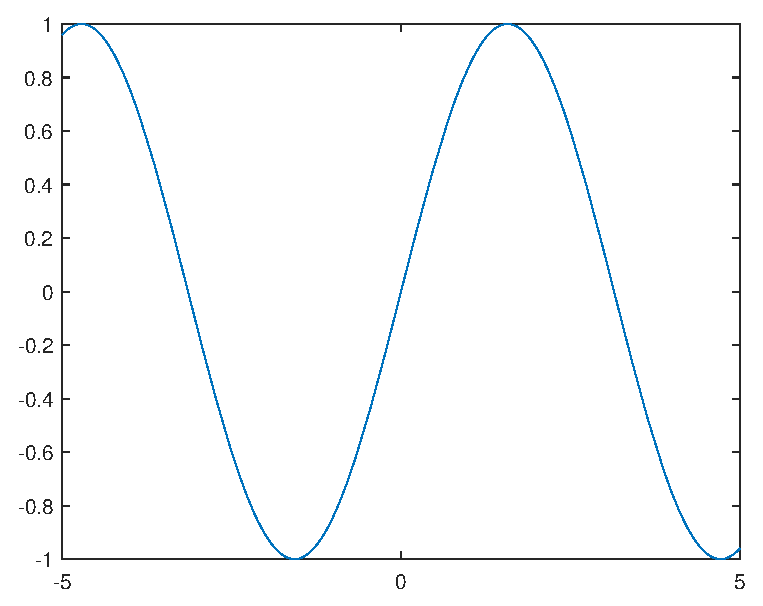
\includegraphics[width=0.48\linewidth]{image1}
  \caption{Example figure using external image files.}
  \label{fig:a}
\end{figure}

\clearpage
The two figures are placed side by side, sharing the same title.
\begin{figure}[htp!]
  \centering
  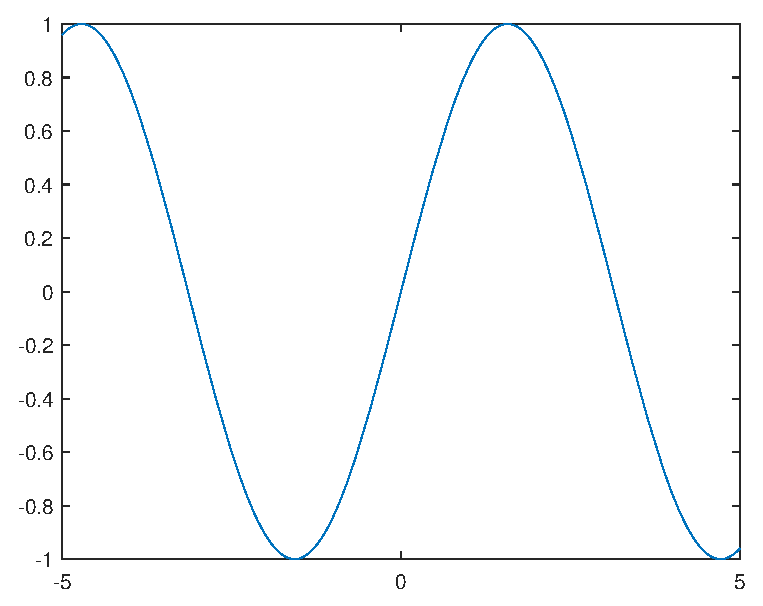
\includegraphics[width=0.45\linewidth]{image1}
  \hfill
  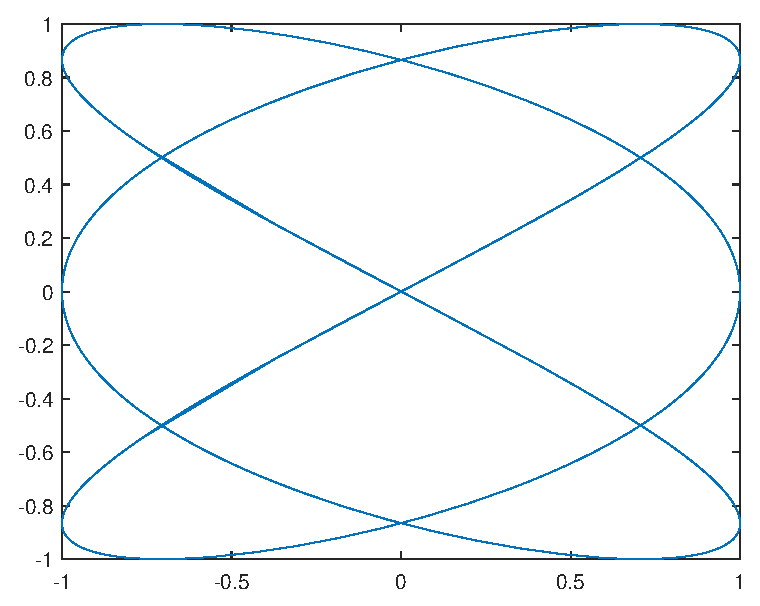
\includegraphics[width=0.45\linewidth]{image2}
  \caption{Left: Caption 1, Right: Caption 2.}
  \label{fig:b}
\end{figure}

Use \texttt{minipage} package to set up images side-by-side, each with its own title.
\begin{figure}[htp!]
\begin{minipage}[t]{0.48\linewidth}
  \centering
  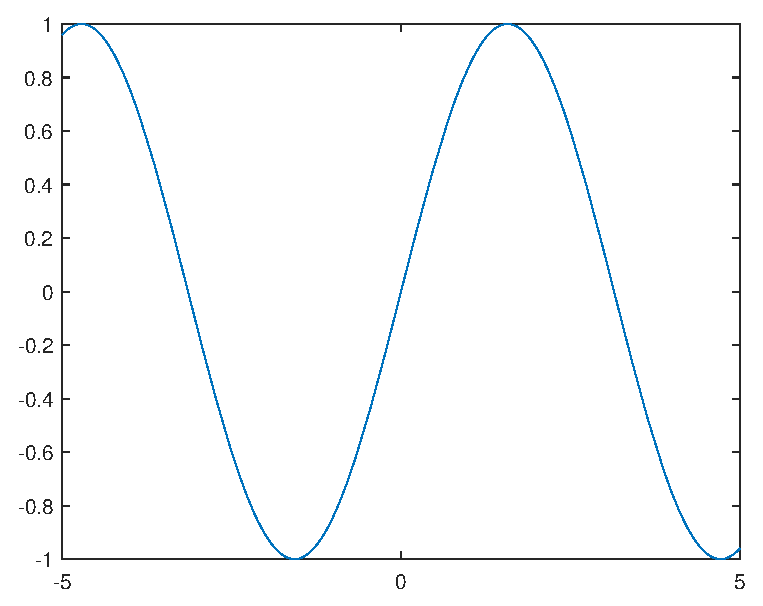
\includegraphics[width=0.96\linewidth]{image1}
  \caption{Caption A}
  \label{fig:image1}
\end{minipage}
\hfill
\begin{minipage}[t]{0.48\linewidth}
\centering
   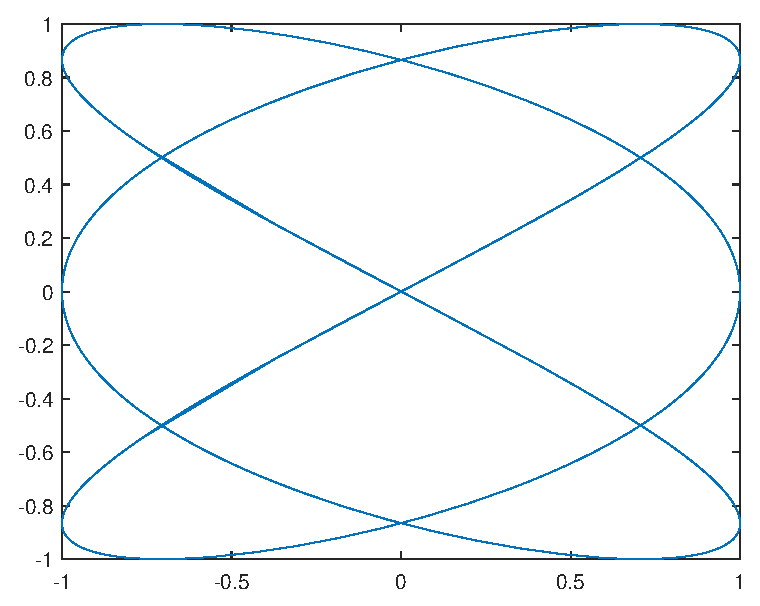
\includegraphics[width=0.95\linewidth]{image2}
   \caption{Caption B}
   \label{fig:image2}
\end{minipage}
\end{figure}




\section{Discussion of \texorpdfstring{{\boldmath$Z=X \cup Y$}}{Z = X union Y}}
\label{sec:discussion}

Some discussions here. Some discussions here. Some discussions here.

\subsection{A sub section}
LaTeX is not a word processor! Instead, LaTeX encourages authors not to worry too much about the appearance of their documents but to concentrate on getting the right content. For example consider this document:

The quick brown fox jumps over the lazy dog. The quick brown fox jumps over the lazy dog. The quick brown fox jumps over the lazy dog. The quick brown fox jumps over the lazy dog. The quick brown fox jumps over the lazy dog. The quick brown fox jumps over the lazy dog. The quick brown fox jumps over the lazy dog.

The quick brown fox jumps over the lazy dog. The quick brown fox jumps over the lazy dog. The quick brown fox jumps over the lazy dog. The quick brown fox jumps over the lazy dog. The quick brown fox jumps over the lazy dog. The quick brown fox jumps over the lazy dog. The quick brown fox jumps over the lazy dog. The quick brown fox jumps over the lazy dog. The quick brown fox jumps over the lazy dog.


\section{The second section}
LaTeX is a high-quality typesetting system; it includes features designed for the production of technical and scientific documentation. \index{LaTeX} is the de facto standard for the communication and publication of scientific documents.

\subsection{A sub section}
LaTeX is not a word processor! Instead, LaTeX encourages authors not to worry too much about the appearance of their documents but to concentrate on getting the right content.

The quick brown fox jumps over the lazy dog. The quick brown fox jumps over the lazy dog. The quick brown fox jumps over the lazy dog. The quick brown fox jumps over the lazy dog. The quick brown fox jumps over the lazy dog. The quick brown fox jumps over the lazy dog. The quick brown fox jumps over the lazy dog. The quick brown fox jumps over the lazy dog. The quick brown fox jumps over the lazy dog.


The quick brown fox jumps over the lazy dog. The quick brown fox jumps over the lazy dog. The quick brown fox jumps over the lazy dog. The quick brown fox jumps over the lazy dog. The quick brown fox jumps over the lazy dog. The quick brown fox jumps over the lazy dog. The quick brown fox jumps over the lazy dog. The quick brown fox jumps over the lazy dog. The quick brown fox jumps over the lazy dog.



\appendix

\chapter{This is the first appendix}

LaTeX is a high-quality typesetting system; it includes features designed
for the production of technical and scientific documentation.
LaTeX is the de facto standard for the communication and publication of scientific documents.
LaTeX is based on the idea that it is better to leave document design to
document designers, and to let authors get on with writing documents.

\section{A sub section}

\begin{equation}\label{eq:abc}
  a^2+b^2=c^2.
\end{equation}

\begin{lemma}
This is a lemma environment.
\end{lemma}

This is Figure \ref{fig:aa}.
\begin{figure}[htp!]
  \centering
  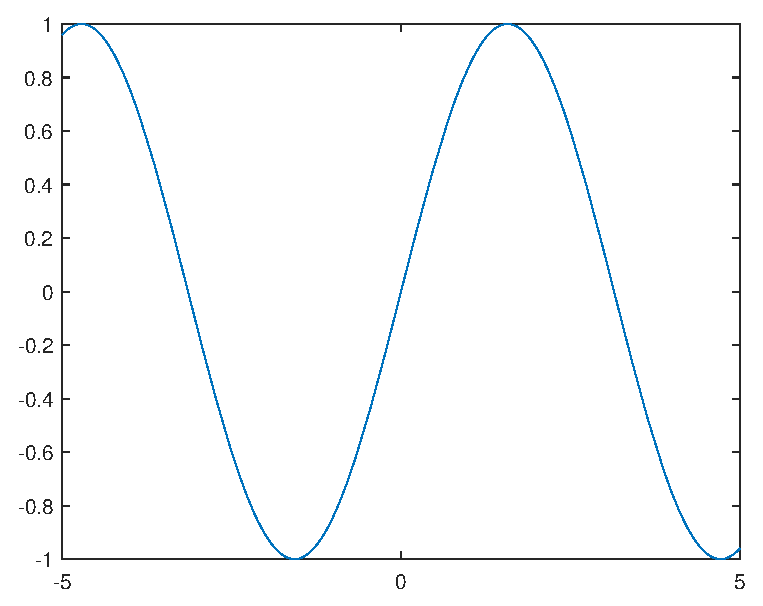
\includegraphics[width=0.48\linewidth]{image1}
  \caption{Example figure using external image files.}
  \label{fig:aa}
\end{figure}

The following table: Table~\ref{tab2:heightweight}. Use \verb|autoref|: \autoref{tab2:heightweight}.

\begin{table}[!htp]
\centering
\renewcommand\arraystretch{1.05}
\caption{A sample of the height and weight of students.}
\label{tab2:heightweight}
% PLCR is defined in the preamble
\begin{tabularx}{0.8\textwidth}{lCCC}
   \toprule %\Xhline{2\arrayrulewidth}
	Number &  Age & Height & Weight\\
	\midrule
	1&14&156&42\\
	2&16&158&45\\
	3&14&162&48\\
	4&15&163&50\\
    \cmidrule{2-4}
	Mean &15&159.75&46.25\\
	\bottomrule
\end{tabularx}
\end{table}

The quick brown fox jumps over the lazy dog. The quick brown fox jumps over the lazy dog. The quick brown fox jumps over the lazy dog. The quick brown fox jumps over the lazy dog. The quick brown fox jumps over the lazy dog. The quick brown fox jumps over the lazy dog. The quick brown fox jumps over the lazy dog. The quick brown fox jumps over the lazy dog. The quick brown fox jumps over the lazy dog.


The quick brown fox jumps over the lazy dog. The quick brown fox jumps over the lazy dog. The quick brown fox jumps over the lazy dog. The quick brown fox jumps over the lazy dog. The quick brown fox jumps over the lazy dog. The quick brown fox jumps over the lazy dog. The quick brown fox jumps over the lazy dog. The quick brown fox jumps over the lazy dog. The quick brown fox jumps over the lazy dog.


The quick brown fox jumps over the lazy dog. The quick brown fox jumps over the lazy dog. The quick brown fox jumps over the lazy dog. Thequick brown \index{fox} jumps over the lazy dog. The quick brown fox jumps over the lazy dog. The quick brown fox jumps over the lazy dog. The quick brown fox jumps over the lazy dog. The quick brown fox jumps over the lazy dog. The quick brown fox jumps over the lazy dog.


The quick brown fox jumps over the lazy dog. The quick brown fox jumps over the lazy dog. The quick brown fox jumps over the lazy dog. The quick brown fox jumps over the lazy dog. The quick brown fox jumps over the lazy dog. The quick brown fox jumps over the lazy dog. The quick brown fox jumps over the lazy dog. The quick brown fox jumps over the lazy dog. The quick brown fox jumps over the lazy dog.


The quick brown fox jumps over the lazy dog. The quick brown fox jumps over the lazy dog. The quick brown fox jumps over the lazy dog. The quick brown fox jumps over the lazy dog. The quick brown fox jumps over the lazy dog. The quick brown fox jumps over the lazy dog. The quick brown fox jumps over the lazy dog. The quick brown fox jumps over the lazy dog. The quick brown fox jumps over the lazy dog.

\section{A sub section}

The quick brown fox jumps over the lazy dog. The quick brown fox jumps over the lazy dog. The quick brown fox jumps over the lazy dog. The quick brown fox jumps over the lazy dog. The quick brown fox jumps over the lazy dog. The quick brown fox jumps over the lazy dog. The quick brown fox jumps over the lazy dog. The quick brown fox jumps over the lazy dog. The quick brown fox jumps over the lazy dog.

The quick brown fox jumps over the lazy dog. The quick brown fox jumps over the lazy dog. The quick brown fox jumps over the lazy dog. The quick brown fox jumps over the lazy dog. The quick brown fox jumps over the lazy dog. The quick brown fox jumps over the lazy dog. The quick brown fox jumps over the lazy dog. The quick brown fox jumps over the lazy dog. The quick brown fox jumps over the lazy dog.


The quick brown fox jumps over the lazy dog. The quick brown fox jumps over the lazy dog. The quick brown fox jumps over the lazy dog. The quick brown fox jumps over the lazy dog. The quick brown fox jumps over the lazy dog. The quick brown fox jumps over the lazy dog. The quick brown fox jumps over the lazy dog. The quick brown fox jumps over the lazy dog. The quick brown fox jumps over the lazy dog.



\chapter{This is the second appendix}
\section{A sub section}

The quick brown fox jumps over the lazy dog. The quick brown fox jumps over the lazy dog. The quick brown fox jumps over the lazy dog. The quick brown fox jumps over the lazy dog. The quick brown fox jumps over the lazy dog. The quick brown fox jumps over the lazy dog. The quick brown fox jumps over the lazy dog. The quick brown fox jumps over the lazy dog. The quick brown fox jumps over the lazy dog.


\section{A sub section}

The quick brown fox jumps over the lazy dog. The quick brown fox jumps over the lazy dog. The quick brown fox jumps over the lazy dog. The quick brown fox jumps over the lazy dog. The quick brown fox jumps over the lazy dog. The quick brown fox jumps over the lazy dog. The quick brown fox jumps over the lazy dog. The quick brown fox jumps over the lazy dog. The quick brown fox jumps over the lazy dog.



\backmatter

\renewcommand{\bibname}{References}

% add References to contents
\clearpage
\phantomsection
\addcontentsline{toc}{chapter}{\bibname}

\bibliographystyle{plain}
\bibliography{reference}


%\begin{thebibliography}{99}
%\bibitem{Adams2003} Adams~R~A, Fournier~J~J~F. Sobolev spaces[M]. Elsevier, 2003.
%
%\bibitem{GoVa2013} Gene~H. Golub and Charles~F. Van~Loan. Matrix computations. The Johns Hopkins University Press, Baltimore, 4th edition, 2013.
%
%\bibitem{Shen1994} Shen~J. Efficient spectral-Galerkin method I. Direct solvers of second- and fourth-order equations using Legendre polynomials[J]. SIAM J. Sci. Comput., 1994, 15(6): 1489-1505.
%
%\bibitem{Tadmor2012} Tadmor~E. A review of numerical methods for nonlinear partial differential
%  equations[J]. Bull. Amer. Math. Soc., 2012, 49(4): 507-554.
%
%\bibitem{TreWei2014} Trefethen~L~N, Weideman~J~A~C. The exponentially convergent trapezoidal rule[J]. SIAM Rev., 2014, 56(3): 385-458.
%
%\end{thebibliography}


\clearpage
\phantomsection
\addcontentsline{toc}{chapter}{\indexname}
\printindex




\end{document}


